\chapter{Funktionalität}
Funktionalität: Spezifikation der einzelnen Produktfunktionen mit genauer und
detaillierter Beschreibung.
\begin{figure}
\begin{center}
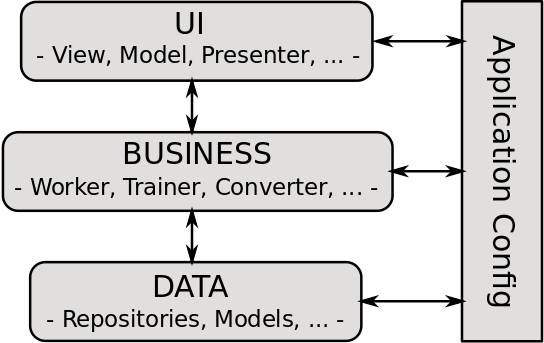
\includegraphics[width=10cm]{Abbildungen/SchichtenModell.png}
\end{center}
\end{figure}

\begin{itemize}
  \item Typische Arbeitsabläufe
  \item Keine Angabe von typischen Verwaltungsfunktionen (CRUD \footnote{Create,
Read, Update, Delete}
\end{itemize}
